\chapter{Design of the Controller}
\label{chap:controller}
This chapter is focused on the controller system of the Media-Online Management system. The controller system is the hand and mouth of the MOM system. Handling the everyday use of the MOM system as activating and restricting usage of media devices.\newline
%This chapter is focused on the controller of the Media-Online Management system. The controller consist of a tag reader and power control device which is discussed in this chapter but when mentioning controller both is implied. \newline
The design and functionality of the prototype controller will be presented in parallel to the designed end product. Meaning we will explain how an optimal solution would look as well as the compromises this project had to reduce to.\newline

\section{Product Design}

The product design section is the vision of the system as a finished product. Figure \ref{fig:Power&Tagdevice} is the illustration of the embedded system called the controller system. The controller system is connected to the server though a Wi-Fi connection to insure that a ethernet outlet don't need to be near every media device. \\ 
The controller consists of two devices, a detection device and power control device.

\begin{figure}[!h]
	\centering
		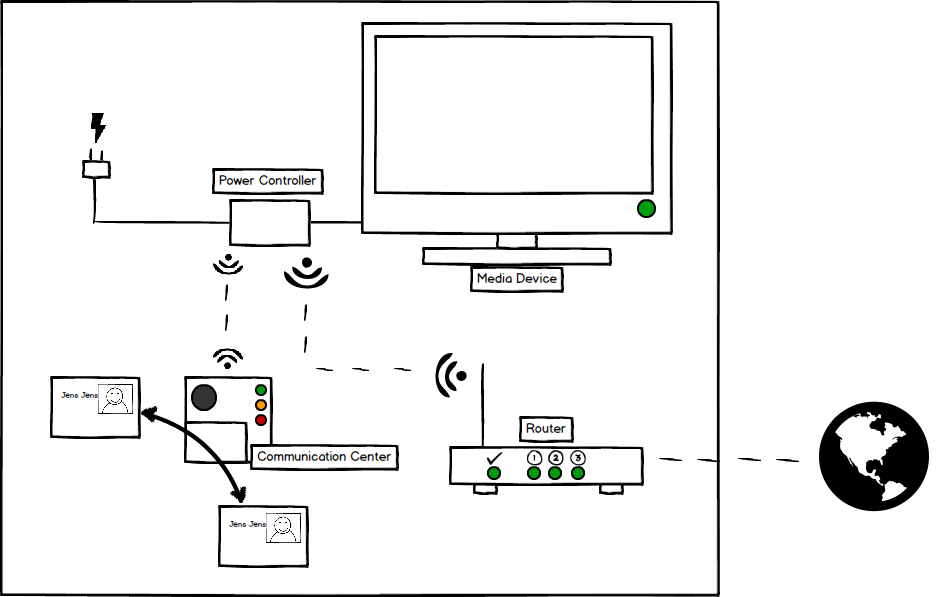
\includegraphics[width=1.00\textwidth]{images/Power&Tagdevice.png}
	\caption{Rich picture for Powercontrol and Tag reader}
	\label{fig:Power&Tagdevice}
\end{figure}

The detection device reads user tags when swiped over the detector device. This device is separated from the power control device to increase user friendliness.\\
The power control device will be placed on the power cable to the media device and will therefor not always be as accessible for use, if one want to scan a tag. Therefor the detection device should be placed in front of the media device to give more user friendliness.\\
%The other device is a powercontrol device which is located on the powerline to the media device and turns on and off the electricity when needed.\newline
The power control device(PCD) is the brain of the two devices and is therefore to monitor the time usage of the media. It should also communicate with the server and detection device. This in our implementation corresponds to the Arduino.\\
The detection device(DD) should also inform the user whom is trying to activate a media of whether the activation has been approved or declined by the server. This in our implementation corresponds to the RFID reader-shield attached to the Arduino.
%The detection device(DD) also works as an information communicator to the user, on the state of the connection to the server about acceptance/decline of log-in. \newline    

\subsection{Scenario Design}
\label{subsec:senarioD}

The system has been designed on multiple scenarios and the criteria of communication to the server and user. 
The controller system have follow functionality: 

\begin{itemize}	
	\item Setup to database server though a Wi-Fi connection. 
	\item Register user tag and get user rights from server. 
	\item Administrate user-rights according to server information.
	\item Monitor the Wi-Fi connection to the server and handle the exception of disconnection. 
	\item Regulate the power to a device recording to the scenario.
	\item Manage the time usage and user restrictions.
	\item Communicate system status to user.
\end{itemize}

The development was done by asking and answering questions to the system in different scenarios.\newline

\paragraph{Setting up and turning on the system.}
In the intended design the PCD will receive the information about the Wi-Fi connection from a USB pen.
If the information on the USB is wrong or not received then a restart button is included to redo the procedure.  \newline
If no error occours, the PCD will connect to the Wi-Fi network and add the controller to the database in the according MOM system. If the connection is not found a message is send to the DD. \newline 
DD indicates that there is no connection by showing a constant red light. The communication protocol can be found in the appendix \vref{appen:lights}.\newline When the connection is established then the DD is ready to read user tags.\newline

However, this design will not be implemented in this project. Due to limitations of available hardware. Instead there is a wired connection to the internet and the controller need to be manually added into the database.

\paragraph{Detection of connection issues and status changes.}
The connection to the sever is tested by a routine call every five minutes from the PCD to the server. In this call the PCD will receive information on when the media should shutdown based on a rule or the user's remaining time. This insures that if any changes occurs to the remaining time or the rules which will influences when the media should shut down will still be handled.
%This insure that there is a connection each five minutes and if any changes in rules or in the time the user may spend on the media. 
In between those calls the PCD will check for a tag from the DD. If the PCD is disconnected from the server the DD is informed so this can be communicated to the user, by use of LED's mounted on the DD.  \newline
	
	

\paragraph{Logon/logoff media device.}
\label{Logonlogoffmedia}
When a tag is read by the DD, the PCD will receive the tag id which is then formed into a log-in message and send to the web servers API. however this is only if no one is already logged on the media device in the MOM system.\\
The PCD will then get a message from the API, about whether the user has permission or not, to use the media. If the user has permission then the PCD should direct power to the media, then save the tag id in local memory and receive the remaining time from the API.\\
The DD should at the same time indicate whether the user is approved to use the media.\\

To log-off the user will swipe ones user tag again and if the PCD receives the same tag id that is stored in the local memory, the PCD will switch off the power to the media and send a log-off message to the API. \\
If another user wants to take over the usage of the media then the PCD should try to log-in with the new tag. If this is declined then the DD should signal this and keep the old user logged on. If it is accepted then the server should finish the first users use and start a new usage log.\\
The PCD will receive the information for the new user without turning the power off and on again.\\
The functionality of switch users is not implemented in the current prototype. Instead it is simply not allowed to logout with another tag, then what was logged in with.\\
%However as a failsafe the system is designed such that if the server does not receive a status update from the controller every five minutes, it will autocratically log the user out, assuming the controller has lost internet connection.


\paragraph{Server disconnection under use.}
\label{sec:ServerDisconnectionUnderUse}
A disconnection from the server is either found under the regular status call after each five minutes or at a log-on/log-off call. A disconnection will lock the device so only the current user can use the media until the PCD is reconnected with the server. The server discovers the lack of connection when there have not been a status call from the device in five minutes. The disconnection is translated to a log-off from the media at the server side. 
The user will not be logged off by the controller but will be able to use his time according to the last status. If the user want to logged off in a period where there is a disconnection, a time stamp is saved and will be sent to the server when the connection is reestablished. The media can also first be used again when the connection is reestablished. 
This procedure have the advantage that the user will not have to cut off the media in use if the connection is unstable. The user will also be able to use another media if it has connection to the server.
The disadvantage is that the user has the possibility to exceed the time restriction if there has been a change in the rules or the user's remaining time. \newline
The implementation of exception made by disconnection in prototype is not as described above.\\
\\
Currently the PCD stores the available amount of time the user currently logged in can keep using the media. 
If the user tries to log out while being disconnected from the server, the PCD keeps trying to log out for five minutes, if this does not succeed it resets itself, knowing the server have handled the problem.\\
However, the last user or a new user can still not log in before the connection is reestablished.\\
\\

Next is a deeper look into how the Arduino works and is setup in our system.